\documentclass[journal, a4paper]{IEEEtran}

\usepackage{xcolor,soul,framed}
\usepackage{graphicx}
\usepackage{url}
\usepackage{xurl}
\usepackage{hyperref}
\usepackage{times}
\usepackage{float}
\usepackage{caption}

\begin{document}

\title{NYC Airbnb Price \& Rating Visualization Report \\ (Data Visualization Final Project)}

\author{
    41247048S Hsieh Yu-Hsuan,
    41247062S Hung Ting-An, \\
    41247006S Chang Cheng-Yi,
    41171218H Huang Yu-Chien
}

\markboth{Data Visualization Final Project (Fallback 2024)}{}

\maketitle

\begin{abstract}
This project aims to explore the distribution, price trends, and their correlation with reviews and geographical locations of NYC Airbnb listings in late 2025 through interactive data visualization techniques. We designed a map visualization system based on Hexagonal Binning to handle a large dataset of approximately 24,091 listings, effectively resolving the issue of overplotting. Enhanced with dynamic filters such as price validation, subway distance, and neighborhood selection, along with statistical charts, the system provides an intuitive and efficient tool for users to explore the data. This report details the data processing workflow, system design philosophy, implementation details, and use case analysis.

\noindent \textbf{GitHub Repository}:
\url{https://github.com/ArthurArthurArthur0817/Data-Visualization}
\end{abstract}

\section{Introduction}
\subsection{Background and Motivation}
Airbnb has become a significant option for modern travel accommodation. However, for tourists, finding a listing that is both affordable, well-rated, and conveniently located is a challenge. As a global tourism hotspot, New York City has a vast and complex distribution of listings, making it difficult to get a comprehensive view through simple list-based searches.

\subsection{Problem Statement and Target Users}
The target users of this project are \textbf{tourists planning to visit NYC} and \textbf{analysts interested in the NYC real estate or hospitality market}.
Our visualization system aims to assist users in three main areas:
\begin{enumerate}
    \item \textbf{Identifying Price Hotspots}: Quickly visualizing which areas are overpriced or affordable.
    \item \textbf{Finding High CP Value Listings}: Combining review counts and prices to find listings that offer great value.
    \item \textbf{Evaluating Transport Convenience}: Filtering listings based on proximity to subway stations, catering to independent travelers.
\end{enumerate}

\section{Data and Data Processing}
\subsection{Data Source}
The data source for this project is \textbf{Inside Airbnb}. We manually downloaded the compressed CSV files for New York City and surrounding areas and placed them in the \texttt{data/raw/} directory. These files were then integrated and preprocessed.
\begin{itemize}
    \item \textbf{Data Volume}: The cleaned dataset contains approximately \textbf{24,091} valid listings.
    \item \textbf{Key Attributes}: Latitude, Longitude, Price, Neighbourhood Group, Room Type, and Number of Reviews.
    \item \textbf{Supplementary Data}: NYC Subway Stations GeoJSON, used to calculate the distance between listings and subway stations.
\end{itemize}

\subsection{Data Preprocessing}
To improve visualization performance and accuracy, we performed the following steps:
\begin{enumerate}
    \item \textbf{Data Cleaning}: Removed invalid data with zero price or abnormal coordinates.
    \item \textbf{Spatial Calculation}: Calculated the straight-line distance from each listing to the nearest subway station and added the \texttt{dist\_to\_subway} attribute for filtering.
    \item \textbf{Hierarchical Structuring}: Established a \textbf{Borough to Neighborhood} hierarchy for the sidebar selection filter.
\end{enumerate}

\section{Target User and Task Requirement}
We defined the following core tasks for our target users:
\begin{itemize}
    \item \textbf{[T1] Distribution Overview}: Users can observe the geographical density distribution of listings on the map.
    \item \textbf{[T2] Price Exploration}: Users can identify regional differences between high and low housing prices.
    \item \textbf{[T3] Conditional Filtering}: Users can filter by budget, room type, and subway distance to narrow down choices.
    \item \textbf{[T4] Details on Demand}: Users can view detailed information such as name and real-time price of specific listings of interest.
    \item \textbf{[T5] Trend Analysis}: Users can compare listing counts and cost-performance ratios across different areas through statistical charts.
\end{itemize}

\begin{figure}[ht]
\centering
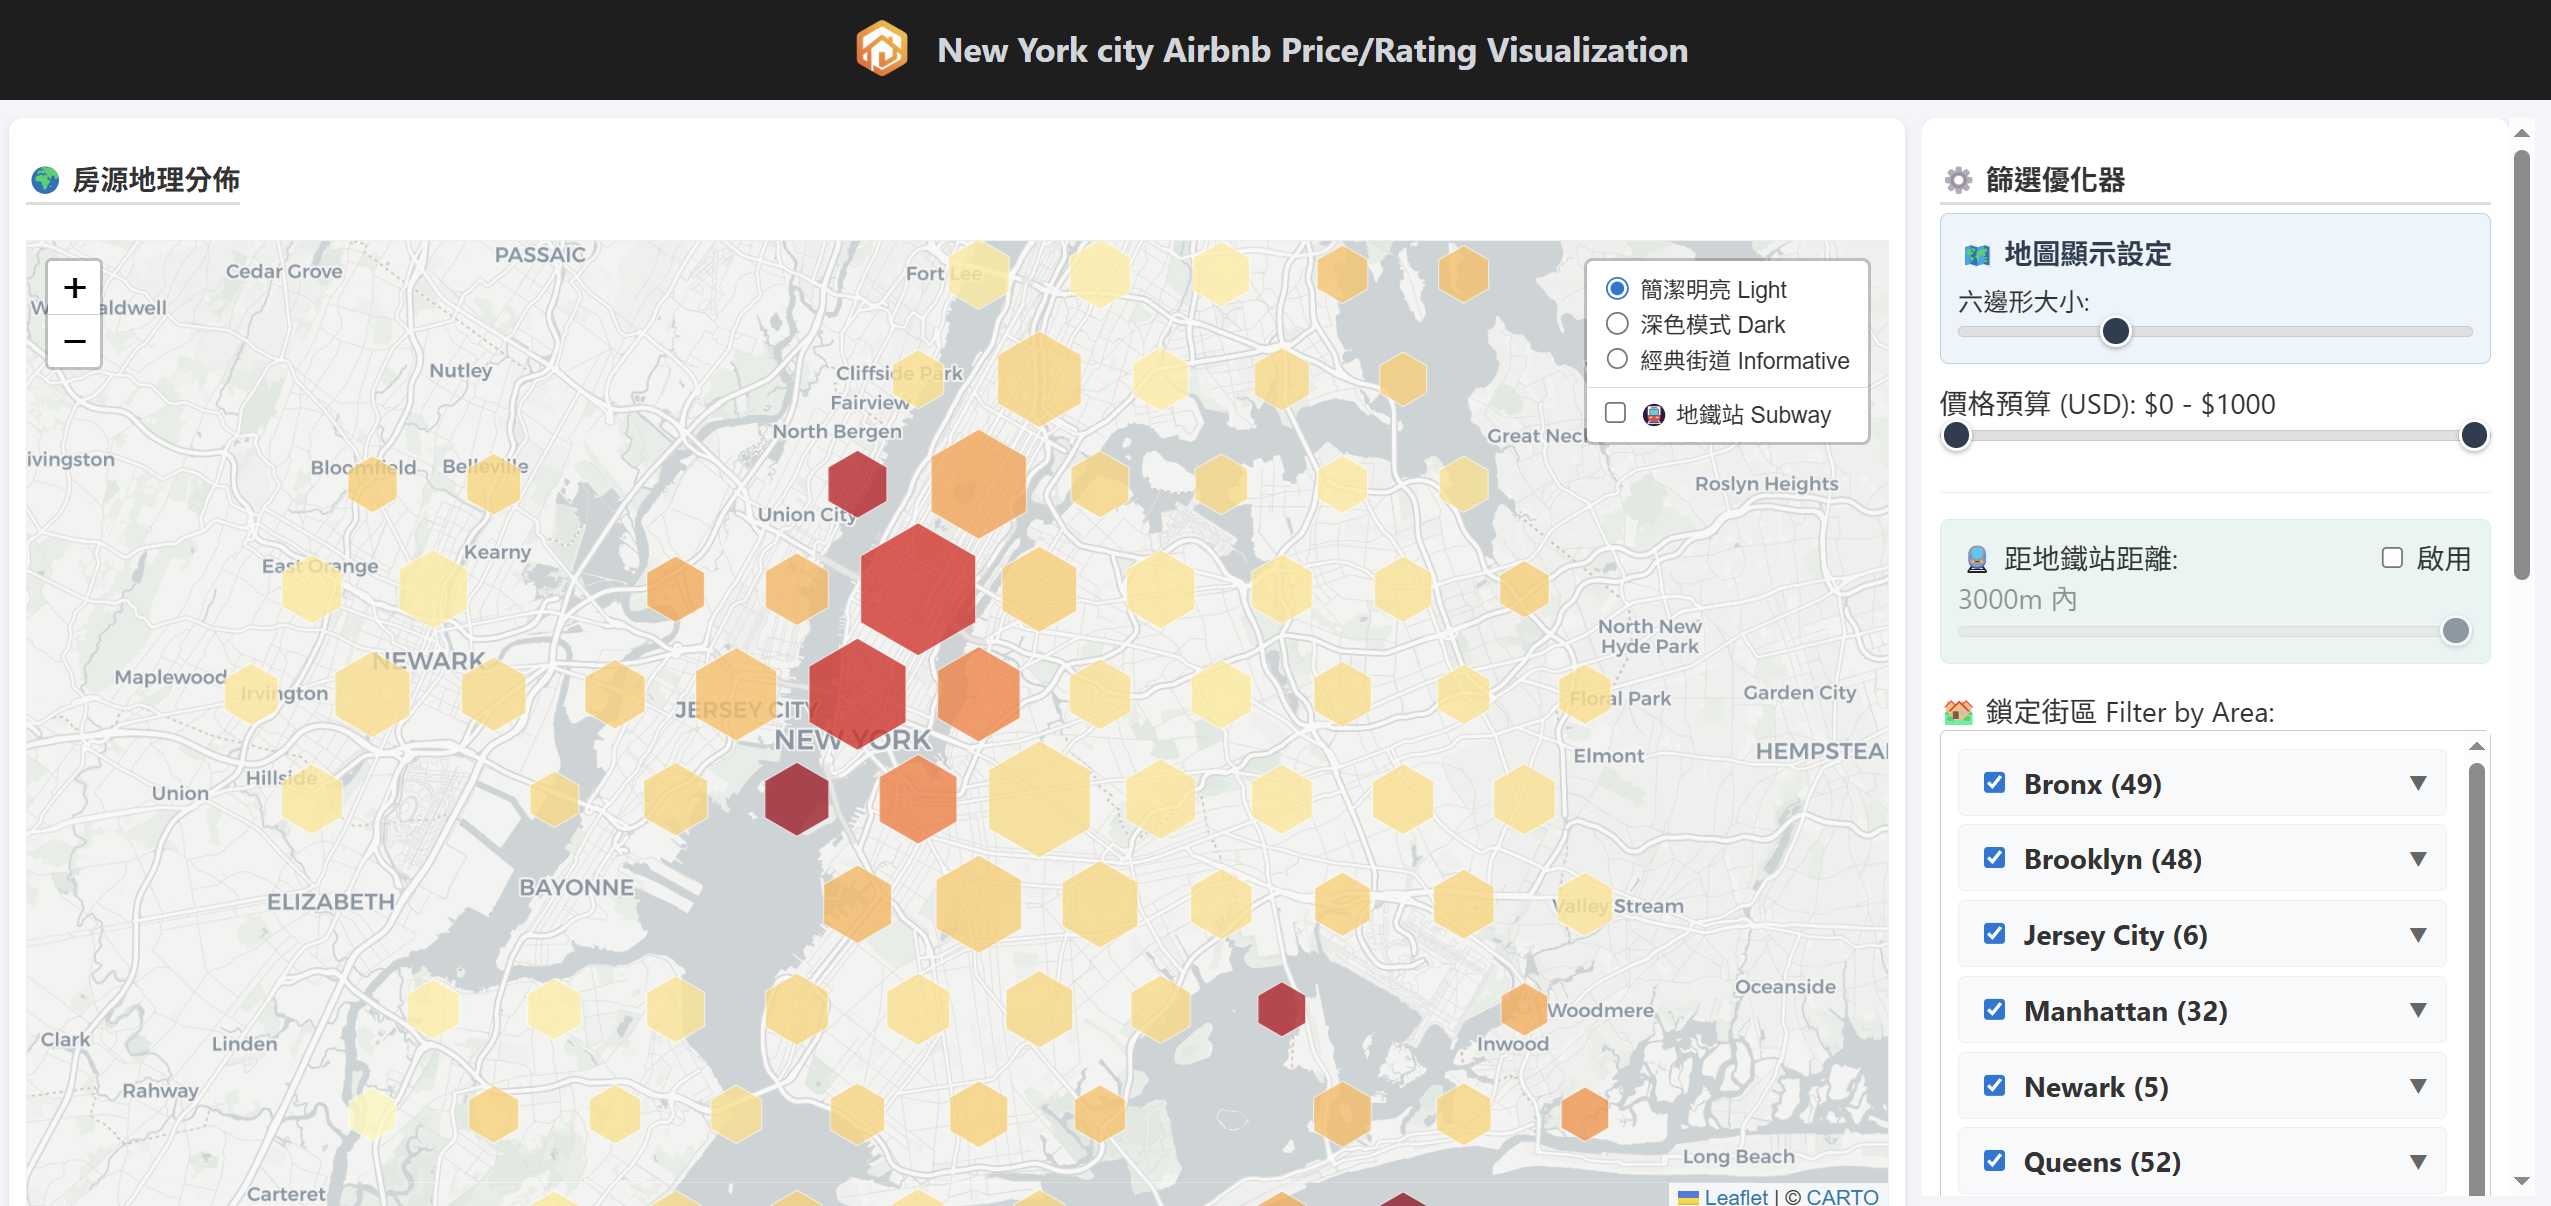
\includegraphics[width=0.95\linewidth]{photo/placeholder_overview.png}
\caption{System Overview with Hexagonal Binning}
\label{fig:overview}
\end{figure}

\clearpage
\section{Visualization Design and Implementation}
The system is built using a \textbf{Web} architecture, utilizing HTML, CSS, and JavaScript, and incorporates \textbf{D3.js} and \textbf{Leaflet.js}.

\subsection{Main Map View}
\begin{itemize}
    \item \textbf{Hexagonal Binning}:
    Since there are over 24,000 listings, plotting all points directly would cause severe \textbf{overplotting}. We used hexagonal binning to aggregate adjacent listings.
    \begin{itemize}
        \item \textbf{Color Encoding}: The shade of the hexagons represents the average price or listing density. Darker colors indicate higher prices or density.
        \item \textbf{Dynamic Radius}: Users can adjust the hexagon size via the right panel to change the aggregation granularity.
    \end{itemize}
    \item \textbf{Semantic Zooming}:
    When users \textbf{Zoom In} to a certain level, the hexagons fade out to reveal individual \textbf{Listing Points}. This allows seamless switching between a macro overview and micro details.
    \item \textbf{Subway Capability Integration}:
    Subway station locations are overlaid on the map, displayed as \textbf{white dots with black borders}, to help reference transport convenience.
\end{itemize}



\subsection{Sidebar Control Panel}
To support task [T3], we designed a robust \textbf{Filter Optimizer} on the right side:
\begin{itemize}
    \item \textbf{Map Display Settings}:
    \begin{itemize}
        \item \textbf{Hexagon Size}: A slider to control aggregation level.
        \item \textbf{Theme Switch}: Provides Light, Dark, and Informative map styles for different contexts.
    \end{itemize}
    \item \textbf{Price Budget}:
    \textbf{Range Slider}, allowing users to set minimum and maximum price limits such as \$100 to \$300.
    \item \textbf{Distance to Subway}:
    Includes an \textbf{Enable Toggle} and a \textbf{Distance Slider}.
    \item \textbf{Filter by Area}:
    \textbf{Hierarchy Checkbox}, listing NYC's five Boroughs and all their subordinate Neighborhoods.
\end{itemize}

\begin{figure}[ht]
\centering
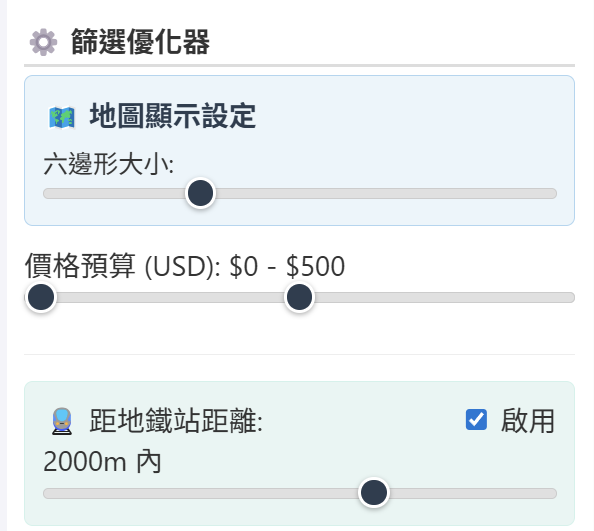
\includegraphics[width=0.8\linewidth]{photo/placeholder_sidebar.png}
\caption{Sidebar Filter Interaction}
\label{fig:sidebar}
\end{figure}

\subsection{Statistical Charts}
The chart area at the bottom right provides analytical perspectives:

\subsubsection{Listing Count Statistics (Bar Chart)}
\begin{itemize}
    \item Shows the total number of listings by Borough or Neighborhood. Users can switch the grouping level.
    \item \textbf{Interaction}: Clicking on a bar zooms the map to that specific area.
\end{itemize}

\begin{figure}[ht]
\centering
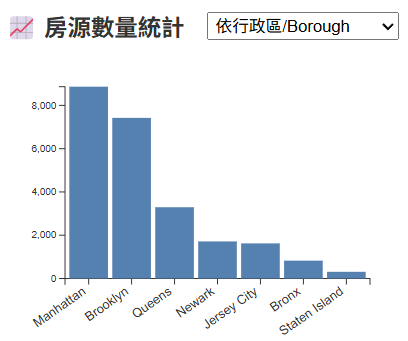
\includegraphics[width=0.95\linewidth]{photo/placeholder_barchart.png}
\caption{Listing Count Bar Chart}
\label{fig:barchart}
\end{figure}

\subsubsection{CP Value Analysis (Price vs Rating Scatter Plot)}
\begin{itemize}
    \item \textbf{X-Axis}: Number of Reviews (popularity). \textbf{Y-Axis}: Price.
    \item \textbf{Color Encoding}: Points are colored by Borough.
    \item \textbf{Interaction}: Supports \textbf{Brush to Filter}. Users can drag a selection box to select a cluster of neighborhoods.
    \item \textbf{Purpose}: Helps identify ``High CP Value'' listings.
\end{itemize}

\begin{figure}[ht]
\centering
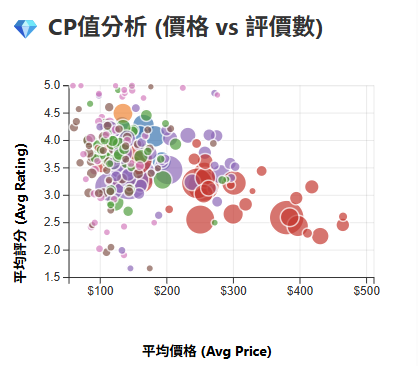
\includegraphics[width=0.85\linewidth]{photo/placeholder_CP-value.png}
\caption{CP Value Analysis}
\label{fig:sidebar}
\end{figure}

\clearpage
\section{Use Cases}
We demonstrate the value of our visualization through two distinct scenarios.

\subsection{Case 1: The Analyst - Discovering High CP Value Neighborhoods}
\textbf{Goal}: Bob wants to know \textbf{``Which neighborhoods offer the best value?''} (High Rating + Low Price).

\begin{figure}[H] 
\centering
\begin{minipage}[b]{0.48\linewidth}
  \centering
  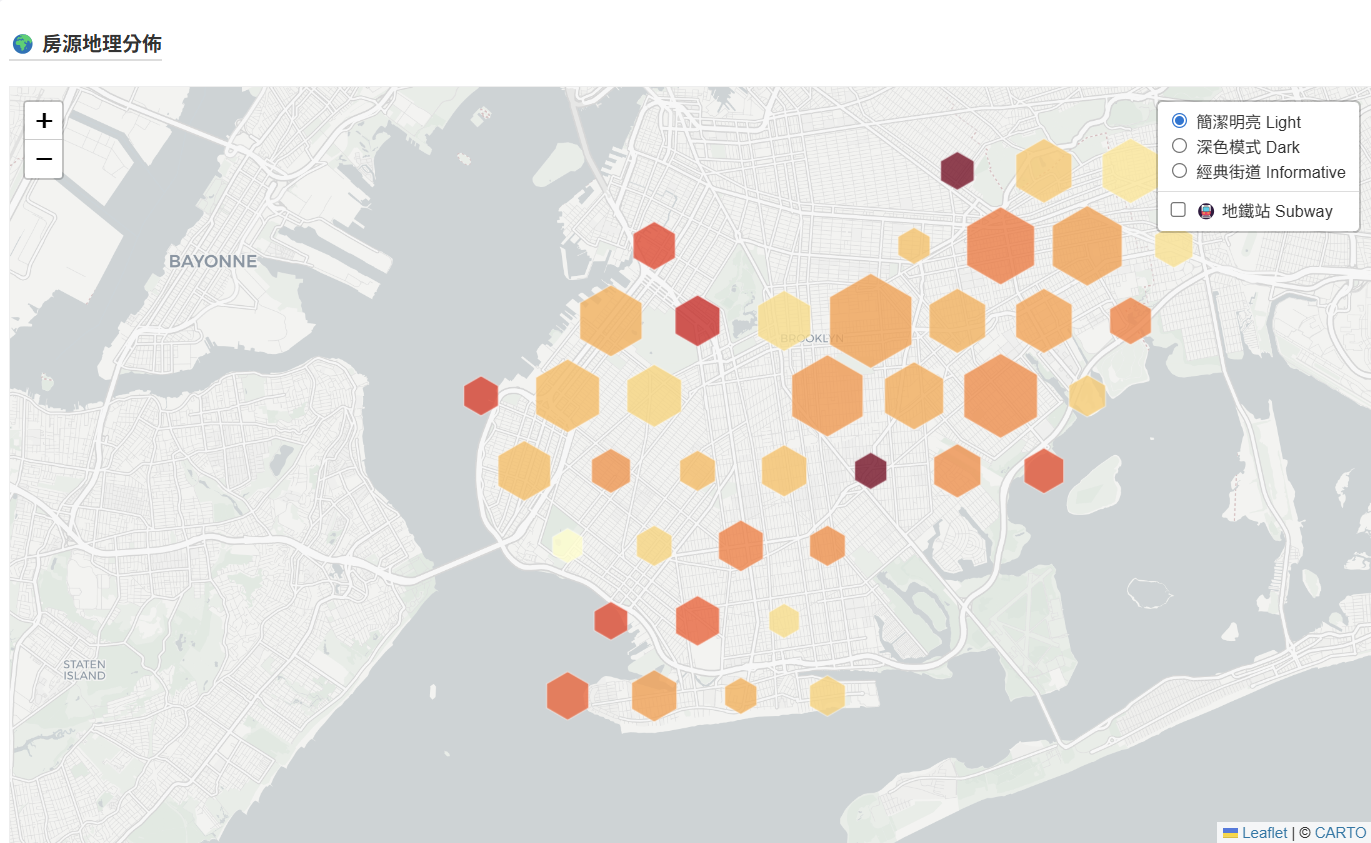
\includegraphics[width=\linewidth]{photo/placeholder_scatterplot_map.png}
  \caption*{(b) Filtered Map}
\end{minipage}
\hfill
\begin{minipage}[b]{0.48\linewidth}
  \centering
  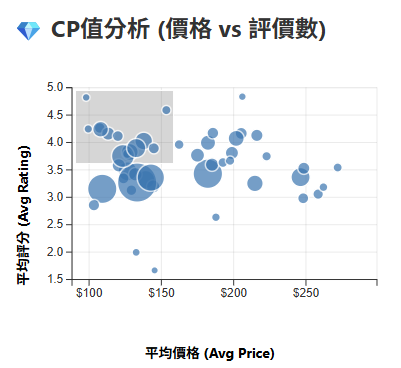
\includegraphics[width=\linewidth]{photo/placeholder_scatterplot_brush.png}
  \caption*{(a) Brush Action}
\end{minipage}

\vspace{0.2cm}

\begin{minipage}[b]{0.48\linewidth}
  \centering
  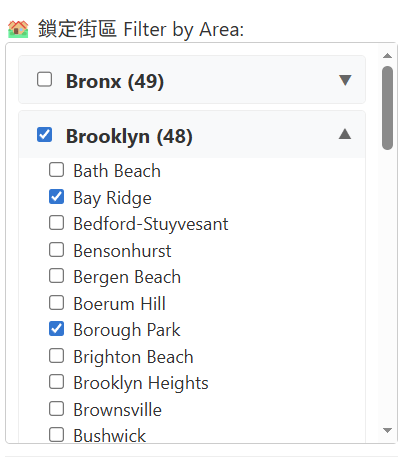
\includegraphics[width=\linewidth]{photo/placeholder_scatterplot_filter.png}
  \caption*{(c) Filter Detail}
\end{minipage}
\hfill
\begin{minipage}[b]{0.48\linewidth}
  \centering
  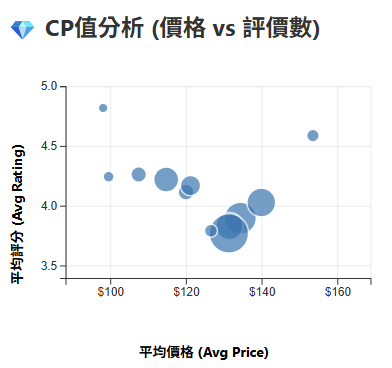
\includegraphics[width=\linewidth]{photo/placeholder_scatterplot_brushed.png}
  \caption*{(d) Selected Result}
\end{minipage}

\caption{Scatter Plot Interaction Flow. (a) User brushes "High Value Zone". (b) Map updates simultaneously. (c) Filter panel syncs. (d) Resulting high-value clusters.}
\label{fig:scatterplot}
\end{figure}

\begin{enumerate}
    \item \textbf{Macro Analysis}: Bob looks at the Scatter Plot.
    \item \textbf{Interaction}: He brushes the ``High Value Zone'' (High Rating > 4.5, Price < \$150) (Fig \ref{fig:scatterplot}a).
    \item \textbf{Insight Discovery}: The map simultaneously filters to show only listings in these clusters (Fig \ref{fig:scatterplot}b).
    \item \textbf{Conclusion}: He discovers high-value listings are concentrated in Astoria and Brooklyn.
\end{enumerate}

\newpage
\subsection{Case 2: The Tourist - Finding ``Hidden Gem'' Accommodation}
\textbf{Goal}: Alice plans to visit NYC with a budget of \$150/night. She wants to stay in \textbf{Brooklyn} but needs to be within walking distance of a subway station.

\begin{figure}[H] 
\centering
\begin{minipage}[c]{0.48\linewidth}
  \centering
  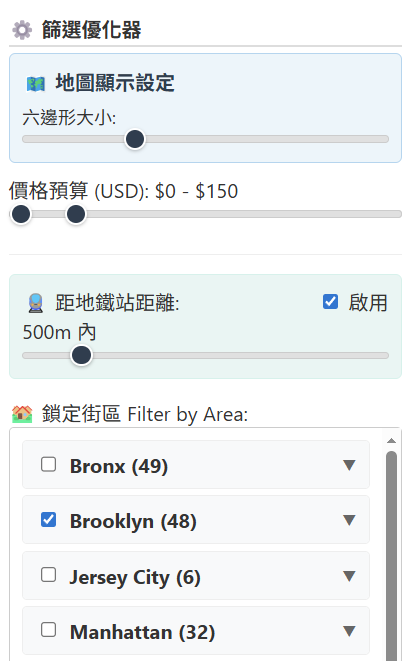
\includegraphics[width=0.95\linewidth]{photo/usecase1_setup.png}
  \caption*{(a) Setup Filters}
\end{minipage}
\hfill
\begin{minipage}[c]{0.48\linewidth}
  \centering
  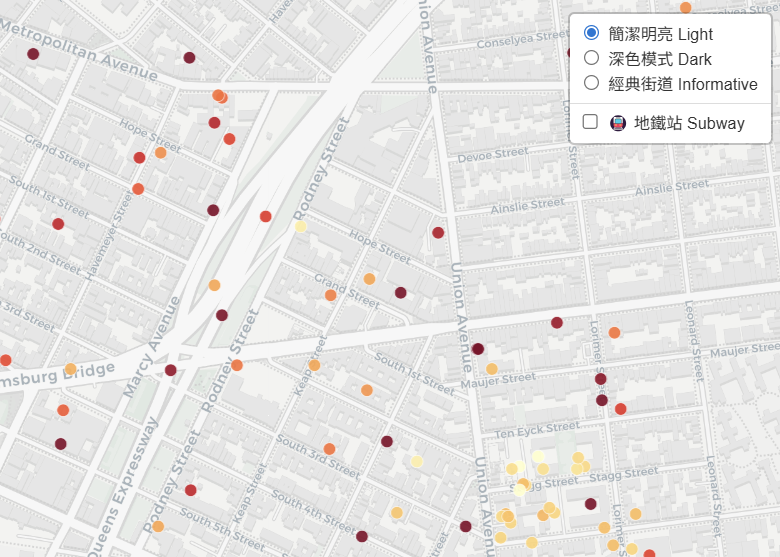
\includegraphics[width=\linewidth]{photo/usecase1_map.png}
  \caption*{(b) Filtered Map Result}
  \vspace{0.2cm} 
  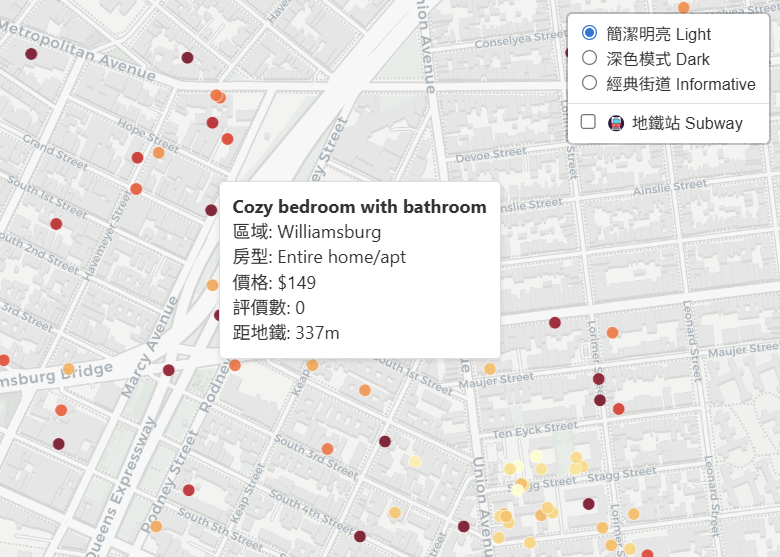
\includegraphics[width=\linewidth]{photo/usecase1_tooltip.png}
  \caption*{(c) Detail Verification}
\end{minipage}

\caption{Use Case 2 Workflow. (a) Filters set for Brooklyn \& Subway. (b) Map shows clusters. (c) Tooltip verifies details.}
\label{fig:usecase}
\end{figure}

\begin{enumerate}
    \item \textbf{Global Filter}: Alice checks ``Brooklyn'' and sets the budget to \$0-\$150.
    \item \textbf{Transport Constraint}: She enables the \textbf{Distance to Subway} toggle (500m) (Fig \ref{fig:usecase}a).
    \item \textbf{Visual Exploration}: She \textbf{zooms in} to Williamsburg (Fig \ref{fig:usecase}b).
    \item \textbf{Detail Verification}: Hovering over points, she finds a \$118 listing with a 4.9-star rating (Fig \ref{fig:usecase}c).
\end{enumerate}

\section{Conclusion and Discussion}
This project successfully implemented a visualization system integrating maps, filters, and statistical charts.
\begin{itemize}
    \item \textbf{Strengths}: Hexagonal binning solves overplotting; multidimensional filters enhance exploration.
    \item \textbf{Limitations}: Static data.
    \item \textbf{Future Work}: Timeline features and real-time APIs.
\end{itemize}

\end{document}